% Ch5.tex

\chapter{Detecting frog calling activity based on acoustic event detection and multi-label learning}
\label{cha:cha7ML}


\section{Overview}
\label{sect:introduction}

This chapter describes the research conducted for detecting frog calling activity (frog abundance and frog species richness). Compared with Chapter \ref{cha:cha6MIML}, acoustic event detection is used to predict the present or absence of eight specific frog species. Here frog abundance is calculated based on the area and content of each segmented event.
In Chapter \ref{cha:cha6MIML}, acoustic features are calculated based on the results of acoustic event detection (AED) to predict frog species richness, but the accuracy of AED results directly affect the multiple-label multiple-instance (MIML) classification performance.
To reduce the bias introduced by AED, this research presents a global feature representation for the classification of recordings with simultaneous vocalising frog species. This feature representation regards all the frog species in each individual recording as a whole. Therefore, the classification process can be framed as multiple-label (ML) learning.  



Compared with that described in Chapter \ref{cha:cha6MIML}, three global feature representations are calculated to classify each segmented recording: linear predictive coding (LPC), MFCCs and wavelet-based features. The wavelet-based features are similar with the features used in Chapter \ref{cha:cha5WaveletFeature}. The difference is that we divide \textit{adaptive WPD sub-band ceptral coefficients} into three equal stages to capture more temporal information.


 
Furthermore, this proposed classification framework is conducted for a long-term analysis. The frog calling activity during the breeding season is calculated. Also, the correlation between the frog calling activity and weather variables is studied for finding the relationship between frog calls and environments. 

  



%In this paper, we proposed a novel method for detecting frog calling activity. Here, frog calling activity, which consists of frog abundance and frog species richness, is detected based on acoustic event detection and multi-label learning. Frog abundance and frog species richness denote the number of individual frog calls and the number of different frog species of each segmented recording, respectively. Specifically, we first sample 10 seconds from every 10-minute recordings. Then, short-time Fourier transform (STFT) is used to obtain a spectrogram for each 10-second recording. Next, acoustic event detection is applied to the spectrogram image for frog abundance detection, which is also used to recognize those recordings without frog calls. Finally, multi-label learning is used to calculate frog species richness with three acoustic features: linear predictive coefficients, Mel-frequency Cepstral coefficients and wavelet-based features. After detecting frog abundance and  frog species richness, statistical analysis is used to find the relationship between frog calling activity (frog abundance and frog species richness) and weather variables (temperature and rainfall). Experiment results show that our proposed method can accurately monitor frog calling activity and reflect its relationship with weather variables.


\section{Materials and methods}
The architecture of this frog calling activity detection system is shown in Figure \ref{fig:Ch7_flowchart}. The system consists of three parts: frog abundance detection, frog species richness detection, and correlation analysis. Each part is discussed in detail in the following subsections.

\begin{figure}[htb!]
\centering
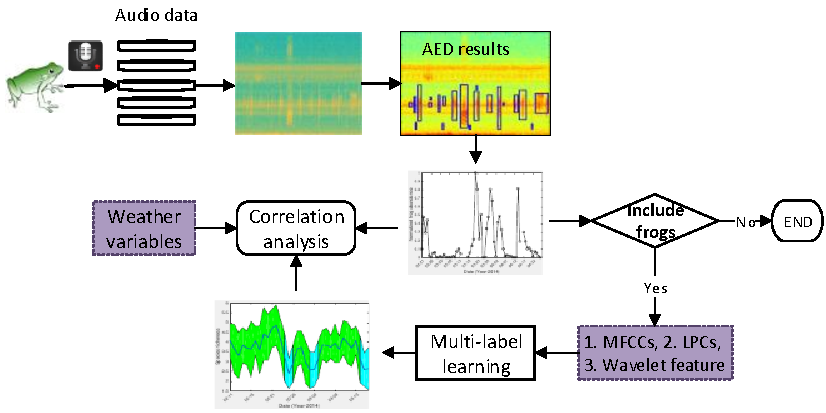
\includegraphics[width=\textwidth]{image/Ch7/flowchart.pdf}
\caption{Flowchart of a frog call classification system using multi-label learning}
\label{fig:Ch7_flowchart}
\end{figure}


\subsection{Acquisition of frog call recordings}
All recordings selected for this chapter were obtained from three sites in Queensland, Australia: \textit{Kiyomi dam}, \textit{Stony creek dam} and  \textit{BG creek dam}, using a battery-powered acoustic sensor (stored in a weather proof metal box) with an external microphone. The recordings were stored on 16 GB SD cards in 64 kbps MP3 mono format. All recordings were collected from February, 2014 to April, 2014, because it is the breeding season in Queensland when male frogs make calls to attract females for the purpose of reproducing. All recordings started around sunset, finished around sunrise every day and have 12 hour duration. This study sampled 10-second recordings every 10 minutes for those continuous recordings. There are 4170, 4908, and 1544 10-second recordings for \textit{Kiyomi dam}, \textit{Stony Creek dam} and \textit{BG Creek dam} respectively, because of data loss. A representative sample of 342 10-second recordings was selected to train and evaluate the proposed method. The ground truth of those 342 10-second recordings is generated by a frog expert, who manually tagged each recording with frog species.

We first manually inspected spectrograms of ten randomly selected call examples for each frog species. Two parameters, dominant frequency and syllable duration, were then measured and averaged, as listed in Table \ref{tab:Ch7_parameters}, which are used as prior information for subsequent analysis.


%the distribution
%of recordings that include the particular frog species and the number of recordings that include
%different number of frog species is shown in Fig.~\ref{fig:labelDistribution}.
\begin{table}[htb!]
\centering
\caption[Acoustic parameters of eight frog species averaged for ten randomly selected syllables]{Dominant frequency ($F_{0}$) and syllable duration ($T_{s}$) of eight frog species averaged for ten randomly selected syllables.}
\label{tab:Ch7_parameters}
\resizebox{0.8\textwidth}{!}{
\begin{tabular}{llcc}
\hline\hline
\textbf{Frog species}       & \textbf{Code} & \multicolumn{1}{l}{\textbf{Dominant frequency (Hz)}} & \textbf{Syllable duration(ms)} \\ \hline
\textit{Canetoad}                    & CAD           & 560                                                          &       NA                     \\ 
\textit{Cyclorana novaehollandiae}   & CNE           & 610                                                          &       400                     \\ 
\textit{Limnodynastes terraereginae} & LTE           & 610                                                          &          100                  \\ 
\textit{Litoria fallax}              & LFX           & 4000                                                         &        280                   \\ 
\textit{Litoria nasuta}              & LNA           & 2800                                                         &       160                      \\ 
\textit{Litoria rothii}             & LRI           & 1800                                                         &        500                    \\ 
\textit{Litoria rubella}             & LRA           & 2300                                                         &       580                     \\ 
\textit{Uperolela mimula}            & UMA           & 2400                                                         &       120                     \\ \hline\hline
\end{tabular}
}
\end{table}

\subsection{Frog abundance monitoring}
Frog abundance is monitored through the detection of acoustic events in a spectrogram image. Here, the spectrogram was generated by applying short-time Fourier transform (STFT) to each 10-second recording. Acoustic event detection, which consists of multiple image processing steps, is modified from our previous study \citep{emr2015Xie} and summarised as follows.
\\
\textbf{Step 1:} Wiener filter 

\noindent To de-noise and smooth the spectrogram, a 2-dimensional Wiener filter is applied to the spectrogram image over a $5 \times 5$ time-frequency grid, where the filter size is selected after the consideration of trade-off between removing the background graininess and blurring acoustic events.
\begin{equation}
\hat{S_{tf}} = \mu + \frac{(\sigma^{2}-\nu^{2})}{\sigma^{2}}(S_{tf}-\nu)
\end{equation}
where $\mu$ and $\sigma^{2}$ are local mean and variance, respectively. $\nu^{2}$ is the noise variance estimated by averaging all local variances. 
\\
\textbf{Step 2:} Spectral subtraction

\noindent After Wiener filtering, the graininess has been removed. However, some noises such as wind, insect, and motor engine, which cover the whole recording, still remained. Here, a modified spectral subtraction is employed for dealing with those noises. Description of this algorithm can be found in our previous study \cite{Xie2016}.

\noindent \textbf{Step 3:} Adaptive thresholding

\noindent Following noise reduction, the next step is to convert the noise reduced spectrogram $\hat{S^{'}_{tf}}$ into the binary spectrogram $S^{b}_{tf}$ for events detection. Here, an adaptive thresholding method named \textit{Otsu thresholding} \cite{otsu1975threshold} is employed to find an optimal threshold.

\begin{equation}
\phi_{b}^{2}(k)=w_{1}(k)w_{2}(k)[\mu_{1}(k)-\mu_{2}(k)]^{2}
\end{equation}
\noindent where $w_{1}(k)=\sum_{0}^{k}p(j)$ is calculated from the histogram as $k$, $p(j)=n(j)/N$ are the values of the normalised gray level histogram, $n(j)$ is the number of values in level $j$, $N$ is the total number of values over the whole spectrogram image, $\mu_{1}(k)=[\sum_{0}^{k}p(j)x(j)]/w_{1}$, $x(j)$ is the value at the centre of the $j$th histogram bin. Then, the threshold, $T_{0}$, is calculated as

\begin{equation}
T_{0}= (\phi_{b1}^{2}(k) + \phi_{b2}^{2}(k)) / 2
\end{equation}

\noindent \textbf{Step 4:} Events filtering using dominant frequency and event area \\
To further remove those events that do not belong to the frog species shown in Table \ref{tab:Ch7_parameters}, dominant frequency ($F_{0}$) and area (number of pixels) within the event boundary ($Ar$) are used for filtering. First, large acoustic events, whose area is larger than $A_{large}$, are separated into small events, because the area of frog calls to be classified in Table \ref{tab:Ch7_parameters} is empirically smaller than $A_{large}$. Then, dominant frequency is used to filter the events. First, the averaged frequency is calculated by averaging the peak frequency within each acoustic event. Then, the event, the averaged frequency of which is not within allowed fluctuation in both sides of dominant frequency, is discarded. Finally, small acoustic events, the area of which are smaller than $A_{small}$, are filtered. Those events, with average frequency of between 300 Hz and 800 Hz, are not filtered out using $A_{small}$, because the area of LTE (averaged frequency is between 300 Hz and 800 Hz) is smaller than $A_{small}$. Figure~\ref{fig:Ch7_AED} shows the acoustic event detection results.




To calculate frog abundance of each segmented recording, the frog abundance is calculated as follows.

\begin{equation}
F_{abun} = \sum_{n=1}^{N}A_{i,j}(n)^2
\end{equation}
Here, $A_{i,j}$ represents the decibel value of location $(i,j)$ within each acoustic event $n$ in the spectrogram.

\begin{figure}
        \centering       
        \begin{subfigure}[b]{0.35\textwidth}
                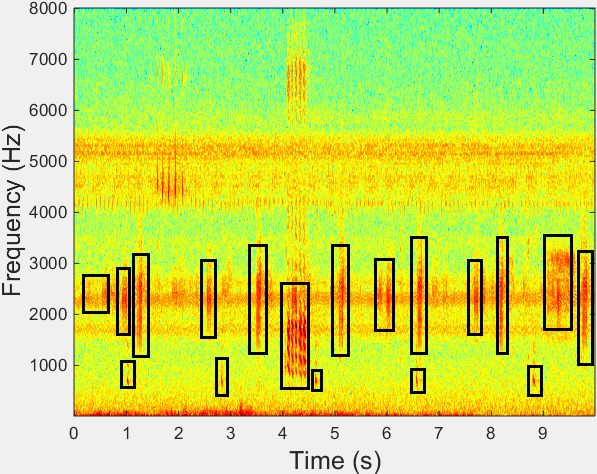
\includegraphics[width=\textwidth]{image/Ch7/spectrogram1-m.png}
                \caption{Baseline}
        \end{subfigure}%
 ~       
        \begin{subfigure}[b]{0.35\textwidth}
                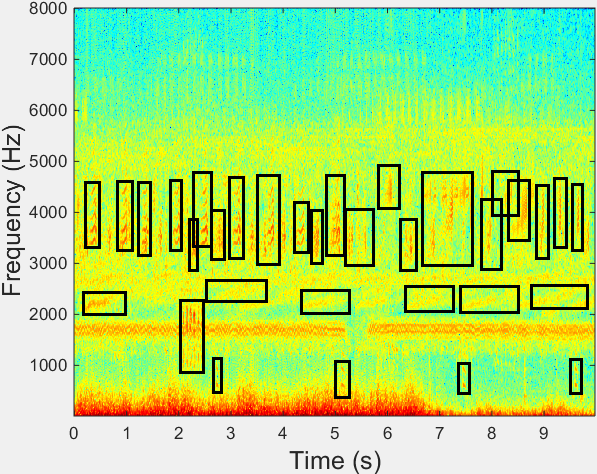
\includegraphics[width=\textwidth]{image/Ch7/spectrogram2-m.png}
                \caption{Baseline}
        \end{subfigure}%
        \\          
        \begin{subfigure}[b]{0.35\textwidth}
                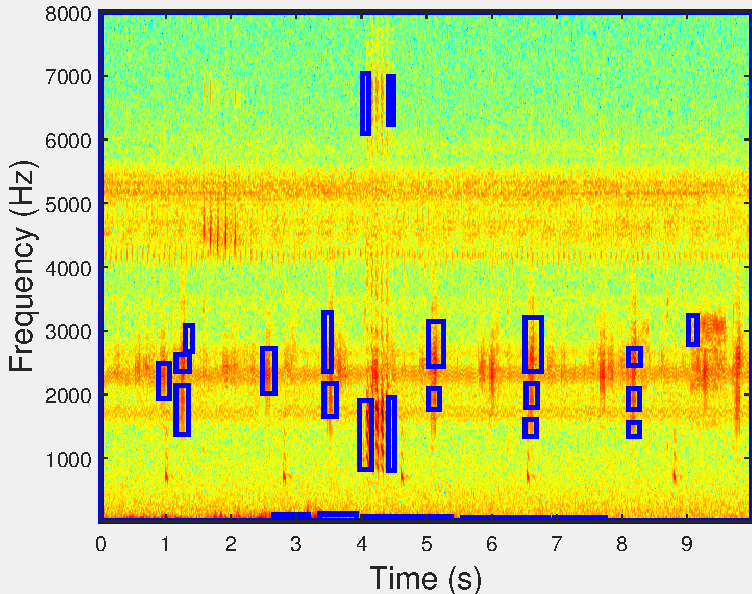
\includegraphics[width=\textwidth]{image/Ch7/AEDFodor.pdf}
                \caption{Method of \cite{fodor2013ninth}}
        \end{subfigure}%
                ~        
        \begin{subfigure}[b]{0.35\textwidth}
                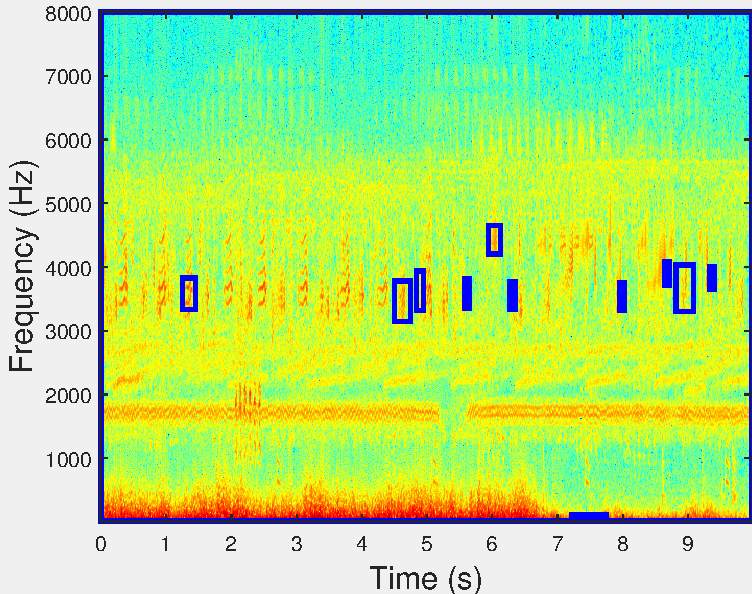
\includegraphics[width=\textwidth]{image/Ch7/AEDFodor_2.pdf}
                \caption{Method of \cite{fodor2013ninth}}
        \end{subfigure}
\\

               \begin{subfigure}[b]{0.35\textwidth}
                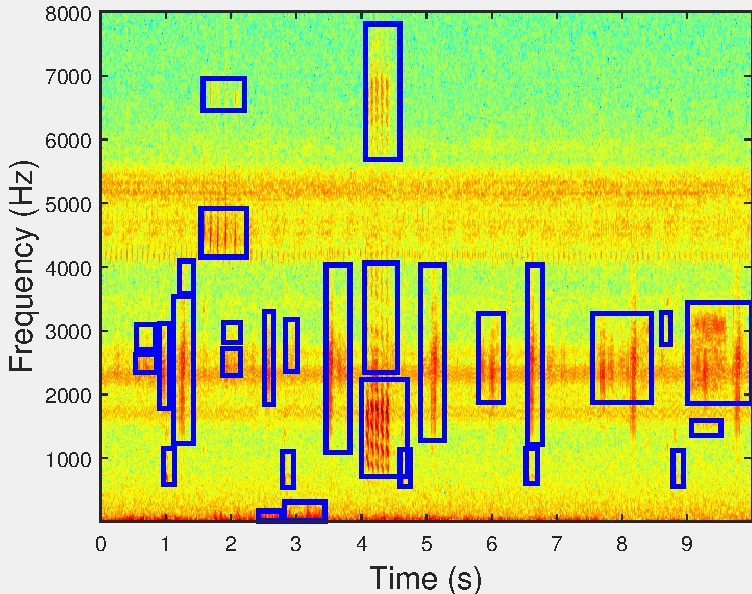
\includegraphics[width=\textwidth]{image/Ch7/AED_Michael.pdf}
                \caption{Method of \cite{Michael2011}}
        \end{subfigure}  
        ~  
                \begin{subfigure}[b]{0.35\textwidth}
                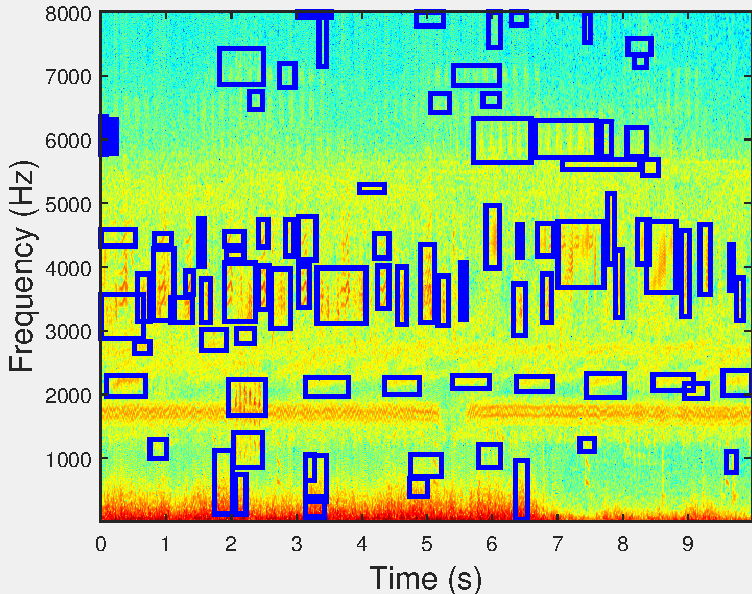
\includegraphics[width=\textwidth]{image/Ch7/AED_Michael_2.pdf}
                \caption{Method of \cite{Michael2011}}
        \end{subfigure}%              
\\         
                \begin{subfigure}[b]{0.35\textwidth}
       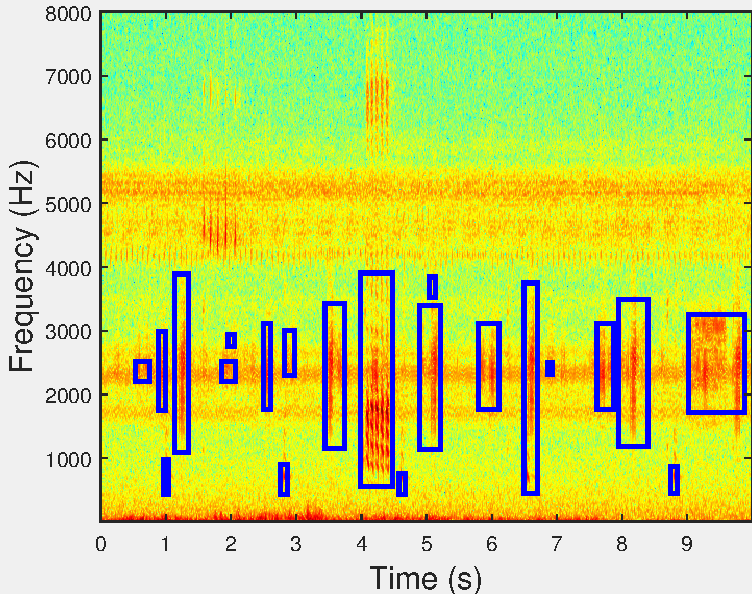
\includegraphics[width=\textwidth]{image/Ch7/AED_Jie.pdf}
                \caption{Proposed method}
        \end{subfigure}     
~
        \begin{subfigure}[b]{0.35\textwidth}
       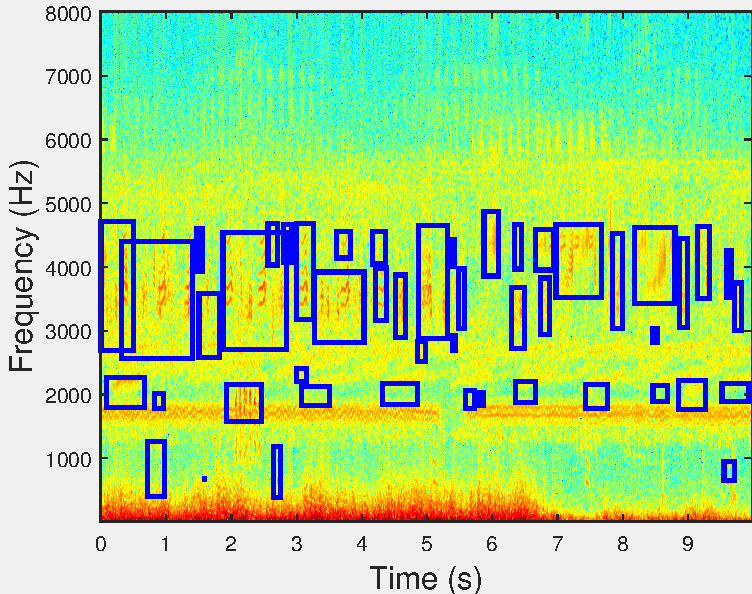
\includegraphics[width=\textwidth]{image/Ch7/AED_Jie_2.pdf}
                \caption{Proposed method}
        \end{subfigure}                
        \caption[Acoustic event detection for frog abundance monitoring using different methods]{Acoustic event detection for frog abundance monitoring using different methods. For each row, different methods are applied to the same recordings. The baseline of the detection results is shown in the first row; detected frog calls are drawn using a blue rectangle. For each column, different methods are used for the same recording.}        
        \label{fig:Ch7_AED}
\end{figure}

\subsection{Wavelet-based feature extraction for species richness analysis}
Frog species richness is calculated by tagging each segmented recording. Since many segmented recordings consist of multiple frog species, one direct solution is to assign each recording with a set of labels (frog species) for explicitly expressing its semantics \cite{ZhangReview2014}. Therefore, multi-label learning is adopted to tag each segmented recording. 

Extracting discriminating
features, which maximise between-group (inter-specie) dissimilarity
and minimise within-group (intra-specie) dissimilarity, is very important for achieving high classification performance \cite{huang2009frog, bedoya2014automatic}. In this chapter, feature extraction is performed based on wavelet packet decomposition using a modified version of the method introduced in Chapter \ref{cha:cha5WaveletFeature} and detailed below. 

For feature extraction, constructing a suitable frequency scale for a wavelet packet (WP) tree based on the dominant frequency of each frog species is the first step, because different frog species tend to have different dominant frequencies \cite{Gingras2013}. In Chapter \ref{cha:cha5WaveletFeature}, k-means clustering was first applied to the extracted dominant frequencies of training data. Then, the frequency scale was built by sorting clustering centroids to construct the WP tree. In this chapter, the prior information on dominant frequency  ($F_{0}$) obtained from Table \ref{tab:Ch7_parameters} is directly used to construct the WP tree. We iteratively detect each WP tree sub-band node until the frequency range of each node includes more than one dominant frequency $F_{0}$. Then, the WP tree of that particular sub-band node will be further split until each sub-band node has only one dominant frequency value or none. After constructing the frequency scale, adaptive frequency scaled wavelet packet decomposition is applied to each segmented recording for feature extraction. 


For each 10-second recording, it is represented as 
$y(n),\,n = 1,...,N$, where $N$ is the length of each recording. Based on the $y(n)$, detailed description for WP-based feature extraction is listed as follows:\\
%\textbf{Step 1}: Add Hamming window to the signal $y(n)$.
%\begin{equation}
%x(n) = w(n)y(n)
%\end{equation}
%\noindent where $w(L)$ is the Hamming window function and defined as $w(n)=0.54-0.46cos(\frac{2n\pi}{L-1}) $, $L$ is the length of Hamming window and set as 512 samples here.
\textbf{Step 1}: Add a Hamming window to the signal y(n) and perform wavelet packet decomposition spaced in adaptive frequency scale as described in \citep{Xie2016}.
\begin{equation}
WP(i,j)=\sum_{i=1}^{M}y(n)w(n)\psi_{(a,b)}(n) 
\end{equation}
\noindent where $w(L)$ is the Hamming window function, $WP(i,j)$ is the wavelet coefficients of the decomposition, $i$ is the sub-band index, $j$ is the index of wavelet coefficients, $\psi_{(a,b)}(n)$ is the wavelet base function, and 'db4' is used experimentally. Here, $a$ and $b$ are the scale and shift parameters, respectively.
\\
\textbf{Step 2}: Calculate the total energy of each sub-band.
\begin{equation}
WP_{i}=\sum_{j=1}^{M_{i}}[WP(i,j)]^2
\end{equation}
\noindent where $i=1,2,...,T$, and $T$ is the total number of sub-band, and $j=1,2,...,M_{i}$, $M_{i}$ is the total number of wavelet coefficients.
\\
\textbf{Step 3}: Normalise the energy of each sub-band.
\begin{equation}
SE_{i}=\frac{WP_{i}}{M_{i}}
\end{equation}
\noindent where $i=1,2,...,T$.
\\
\textbf{Step 4}: Perform discrete cosine transform on the logarithm sub-band energy for dimension reduction and obtain the WP-based feature.
\begin{equation}
WP_{base}(d)=\sum_{i=1}^{T}logSE_{i}cos(\frac{d(i-0.5)}{T}\pi)
\end{equation}
\noindent where $d=1,2,...,d^{'}$, $1 \leq d^{'} \leq T$, here $d^{'}$ is the dimension of  WP-based feature, and set as 12. 

Differently from that described in Chapter \ref{cha:cha5WaveletFeature}, the recording is first segmented into frames using a Hamming window. Then, all frames are divided into three equal parts, and the WP-feature within each part is averaged, respectively, because different frog species within similar frequency bands may exist in one 10-second recording, segmenting each recording into small parts might be able to keep the information of different frog species in the same frequency band. Besides the WP-based feature, two other acoustic features, linear predictive coefficients (LPCs) and Mel-frequency Cepstral coefficients (MFCCs), are calculated for the comparison.




\subsection{Multi-label classification for species richness analysis} 
Since many segmented recordings consist of calls from multiple frog species, frog call classification can be framed as a multi-label classification problem. However, previous studies have not adopted multi-label learning to classify frog calls. Therefore, it is worth investigating different multi-label learning algorithms for the classification of multiple vocalising frog species. In this chapter, four multi-label learning algorithms, whose base classifier is a C4.5 decision tree, are employed: binary relevance (BR), classifier chains (CC), random k-labEL Pruned Sets (RAKEL and RAKEL1) \cite{ZhangReview2014}. The default parameter settings of those four multi-label learning algorithms are used. The trained classifier, which achieves the best classification performance, is then used to tag the rest recordings. After tagging each 10-second recording, frog species richness is lastly calculated as follows.

\begin{equation}
F_{rich} = \frac{\sum_{k=1}^{K}f_{rich}(k)}{K}
\end{equation} 
where $f_{rich}(k)$ is the number of frog species of each tagged 10-second recording, $K$ is the number of 10-second recording for each day.




\section{Experiment results}



\subsection{Experiment setup}
Each 10-second recording is divided into frames of 512 samples and 50\% frame overlap for STFT. $A_{large}$ and $A_{small}$, which are used for area filtering in acoustic event detection, are empirically set at 3000 pixels and 300 pixels, respectively. Allowed fluctuations in both sides of dominant frequency are 300 Hz for dominant frequency filtering. For WP-based feature, window size and overlap are 512 samples and 50\%, the window function is a Hamming window. All algorithms were programmed in Matlab 2014b except multi-label learning, which was implemented in Meka 1.7.7\footnote[4]{http://meka.sourceforge.net/}. 




\subsection{Frog abundance detection}
Figure~\ref{fig:frogAbundance} shows the frog abundance result of three selected sites through the whole frog breeding season. It can be found that the frog abundance of the same site changes a great deal over time. In the \textit{Kiyomi dam}, frog abundance is relatively high from February 21 to February 25. However, frog abundance is quite low in two periods, which are February 26 to March 11 and April 07 to April 12. The highest abundance of this site is achieved on March 22. However, the highest abundance for \textit{Stony Creek dam} and \textit{BG Creek dam} is obtained in February, which shows that frog abundance of different sites often varies a lot for different environments. Recordings of 47 days of all three sites have no frog calls. In the subsequent analysis, only those recordings that consist of frog calls are used for frog species richness analysis. 

\begin{figure}[htb!]
\centering
        \begin{subfigure}[b]{0.3\textwidth}
                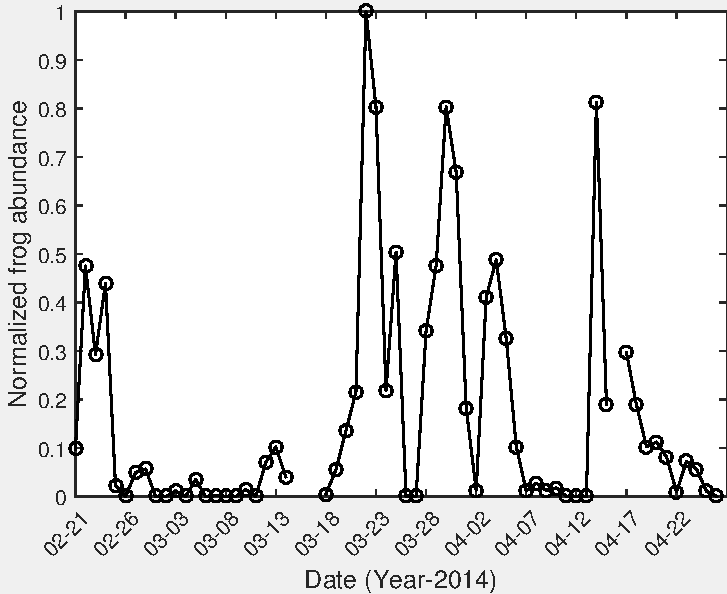
\includegraphics[width=\textwidth]{image/Ch7/abundance1075.pdf}
                \caption{\textit{Kiyomi dam}}
        \end{subfigure}
       ~
              \begin{subfigure}[b]{0.3\textwidth}
                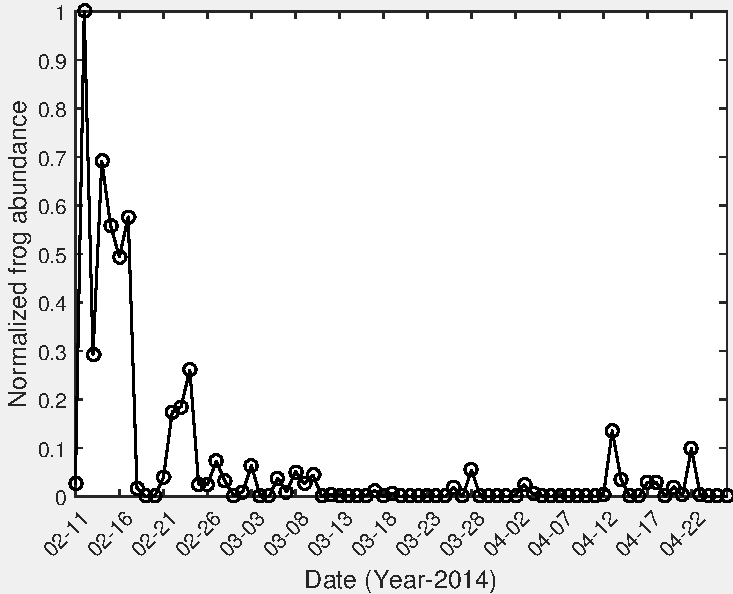
\includegraphics[width=\textwidth]{image/Ch7/abundance1078.pdf}     
                \caption{\textit{Stony creek dam}}           
        \end{subfigure} 
               ~
              \begin{subfigure}[b]{0.3\textwidth}
                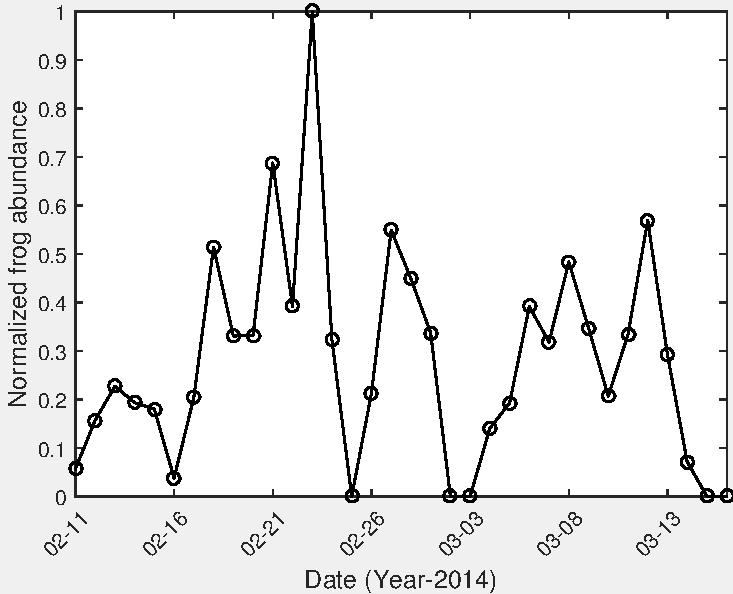
\includegraphics[width=\textwidth]{image/Ch7/abundance1079.pdf}     
                \caption{\textit{BG creek dam}}           
        \end{subfigure}       
\caption[Frog abundance detection of different sites]{Frog abundance detection of different sites: \textit{Kiyomi dam}, \textit{Stony Creek dam} and \textit{BG Creek dam}. For \textit{Kiyomi dam}, three days do not record any acoustic data and then there is no value in those particular days. All the frog abundance value is normalised to [0 1].}
        \label{fig:frogAbundance}
\end{figure}



\subsection{Frog species richness analysis}
Different multi-label learning algorithms are applied on 342 selected recordings to compare different feature sets. Then, six evaluation rules are used to compare the performance with the combination of four feature sets and four multi-label algorithms: Hamming loss, Rank loss, Average precision, One error, Exampled based F1, and Micro F1 \cite{Madjarov20123084, ZhangReview2014}. 
Experiment results are shown in Table~\ref{tab:classificationResults}.

%\vspace{-1em}
\begin{table}[htb!]
\centering
\caption[Classification results based on four feature sets and four multi-label learning algorithms.]{Classification results based on four feature sets and four multi-label learning algorithms. Here the methods for multi-label algorithms are in accordance to the name in the Meka software. The base classifier of all methods is decision tree. For a metric, the best value is in bold. Here, $\downarrow$ indicates ‘the smaller the better’, while ‘$\uparrow$’ indicates ‘the bigger the better’.}
\label{tab:classificationResults}
\resizebox{\textwidth}{!}{
\begin{tabular}{llllllll}
\hhline{========}
\textbf{Features}                  & \textbf{Method} & \textbf{Hamming loss} $\downarrow$ & \textbf{Rank loss} $\downarrow$ & \textbf{Average precision} $\uparrow$& \textbf{One error} $\downarrow$& \textbf{Exampled based F1} $\uparrow$ & \textbf{Micro F1} $\uparrow$ \\ \hline
MFCCs+LPCs                & BR              & 0.155 $\pm$ 0.015           & 0.171 $\pm$ 0.037        & \textbf{0.446 $\pm$ 0.061}                & 0.246 $\pm$ 0.063        & 0.699 $\pm$ 0.03                 & 0.749 $\pm$ 0.024       \\ 
                          & CC              & 0.147 $\pm$ 0.018           & 0.147 $\pm$ 0.02         & 0.35 $\pm$ 0.016                 & 0.199 $\pm$ 0.042        & 0.722 $\pm$ 0.035                & 0.756 $\pm$ 0.029       \\ 
                          & RAKEL           & 0.167 $\pm$ 0.038           & 0.122 $\pm$ 0.026        & 0.333 $\pm$ 0.017                & 0.194 $\pm$ 0.063        & 0.721 $\pm$ 0.044                & 0.752 $\pm$ 0.041       \\ 
                          & RAKEL1           & 0.134 $\pm$ 0.012           & 0.099 $\pm$ 0.025        & 0.342 $\pm$ 0.023                & \textbf{0.147 $\pm$ 0.056}        & 0.74 $\pm$ 0.044                 & 0.783 $\pm$ 0.022       \\ 
Multi-stage MFCCs + LPCs  & BR              & 0.155 $\pm$ 0.016           & 0.169 $\pm$ 0.035        & 0.445 $\pm$ 0.062                & 0.249 $\pm$ 0.064        & 0.7 $\pm$ 0.03                   & 0.75 $\pm$ 0.024        \\ 
                          & CC              & 0.147 $\pm$ 0.018           & 0.147 $\pm$ 0.021        & 0.35 $\pm$ 0.016                 & 0.199 $\pm$ 0.042        & 0.722 $\pm$ 0.034                & 0.756 $\pm$ 0.028       \\ 
                          & RAKEL           & 0.166 $\pm$ 0.035           & 0.124 $\pm$ 0.027        & 0.334 $\pm$ 0.018                & 0.194 $\pm$ 0.069        & 0.724 $\pm$ 0.048                & 0.754 $\pm$ 0.04        \\ 
                          & RAKEL1           & 0.134 $\pm$ 0.013           & 0.101 $\pm$ 0.026        & 0.342 $\pm$ 0.02                 & 0.15 $\pm$ 0.063         & 0.737 $\pm$ 0.05                 & 0.783 $\pm$ 0.023       \\ 
WP-based feature + LPCs             & BR              & 0.148 $\pm$ 0.025           & 0.139 $\pm$ 0.033        & 0.356 $\pm$ 0.065                & 0.254 $\pm$ 0.063        & 0.708 $\pm$ 0.046                & 0.762 $\pm$ 0.036       \\ 
                          & CC              & 0.168 $\pm$ 0.031           & 0.168 $\pm$ 0.045        & 0.341 $\pm$ 0.027                & 0.272 $\pm$ 0.061        & 0.684 $\pm$ 0.054                & 0.723 $\pm$ 0.048       \\ 
                          & RAKEL           & 0.155 $\pm$ 0.023           & 0.103 $\pm$ 0.022        & 0.324 $\pm$ 0.018                & 0.178 $\pm$ 0.031        & 0.729 $\pm$ 0.032                & 0.763 $\pm$ 0.030       \\ 
                          & RAKEL1           & 0.14 $\pm$ 0.027            & 0.094 $\pm$ 0.018        & 0.333 $\pm$ 0.028                & 0.193 $\pm$ 0.063        & 0.727 $\pm$ 0.053                & 0.773 $\pm$ 0.042       \\ 
Multi-stage WP-based feature + LPCs & BR              & 0.153 $\pm$ 0.014           & 0.147 $\pm$ 0.022        & 0.364 $\pm$ 0.056                & 0.266 $\pm$ 0.037        & 0.689 $\pm$ 0.035                & 0.75 $\pm$ 0.025        \\ 
                          & CC              & 0.142 $\pm$ 0.029           & 0.146 $\pm$ 0.023        & 0.345 $\pm$ 0.019                & 0.254 $\pm$ 0.094        & 0.714 $\pm$ 0042                 & 0.764 $\pm$ 0.045       \\ 
                          & RAKEL           & 0.154 $\pm$ 0.022           & 0.11 $\pm$ 0.012         & 0.33 $\pm$ 0.027                & 0.196 $\pm$ 0.062        & 0.739 $\pm$ 0.022                & 0.768 $\pm$ 0.025       \\ 
                          & RAKEL1           & \textbf{0.131 $\pm$ 0.012          } & \textbf{0.09 $\pm$ 0.014}         & 0.33 $\pm$ 0.026                 & 0.173 $\pm$ 0.03         & \textbf{0.743 $\pm$ 0.026}               & \textbf{0.787 $\pm$ 0.018}       \\ \hhline{========}
\end{tabular}
}
\end{table}




The combination of multi-stage WP-based feature+LPCs and the RAKEL1 method achieves the best performance. Therefore, this combination is used for the testing data. 
Figure~\ref{fig:frogRichness} shows the frog species richness of the three selected sites. For all the three sites, the variation of species richness is not high, which shows that species richness of the same area is relatively stable. However, frog species richness of \textit{BG Creek dam} has a smaller variation over the time than \textit{Kiyomi dam} and \textit{Stony Creek dam}. The comparison of the species richness for the three sites is shown in Figure~\ref{fig:richnessSite}. In contrast to other sites, the species richness in \textit{BG Creek dam} is the highest. This might be that \textit{BG Creek dam} is closer to a river and farther away from the human community.


\begin{figure}[htb!]
\centering
        \begin{subfigure}[b]{0.3\textwidth}
                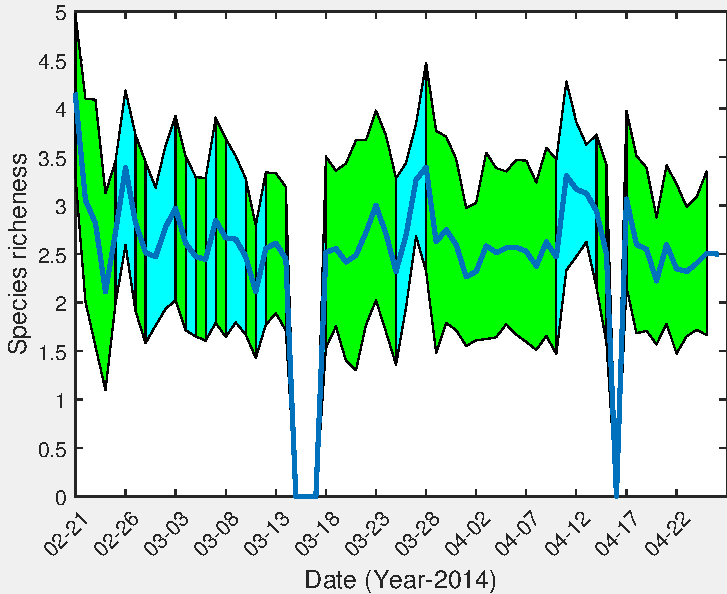
\includegraphics[width=\textwidth]{image/Ch7/richness1075.pdf}
                \caption{\textit{Kiyomi dam}}
        \end{subfigure}
       ~
              \begin{subfigure}[b]{0.3\textwidth}
                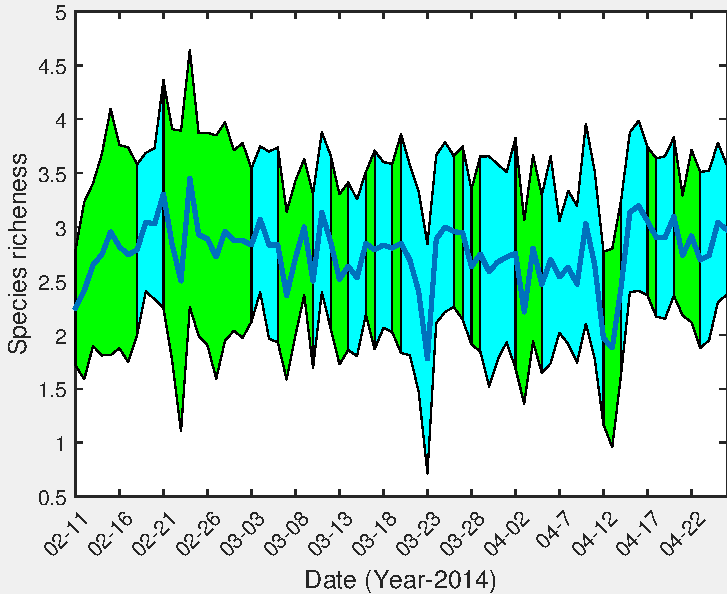
\includegraphics[width=\textwidth]{image/Ch7/richness1078.pdf}     
                \caption{\textit{Stony creek dam}}           
        \end{subfigure} 
        ~
              \begin{subfigure}[b]{0.3\textwidth}
                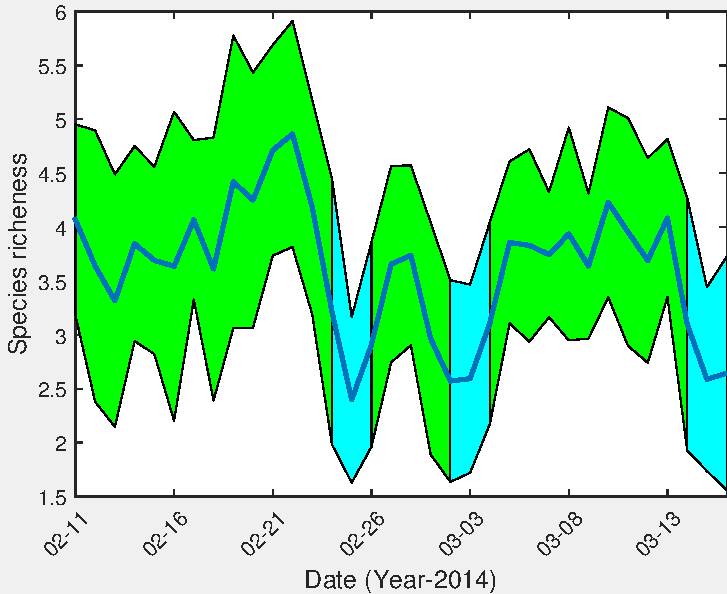
\includegraphics[width=\textwidth]{image/Ch7/richness1079.pdf}     
                \caption{\textit{BG creek dam}}           
        \end{subfigure}       
\caption[Frog species richness distribution of three selected sites]{Frog species richness distribution of three selected sites. Here green bar represents the species variation, blue bar means there is no frog calls, zero value denotes the data loss of those particular days.}
        \label{fig:frogRichness}
\end{figure}

\begin{figure}[htb!]
	\begin{centering}
	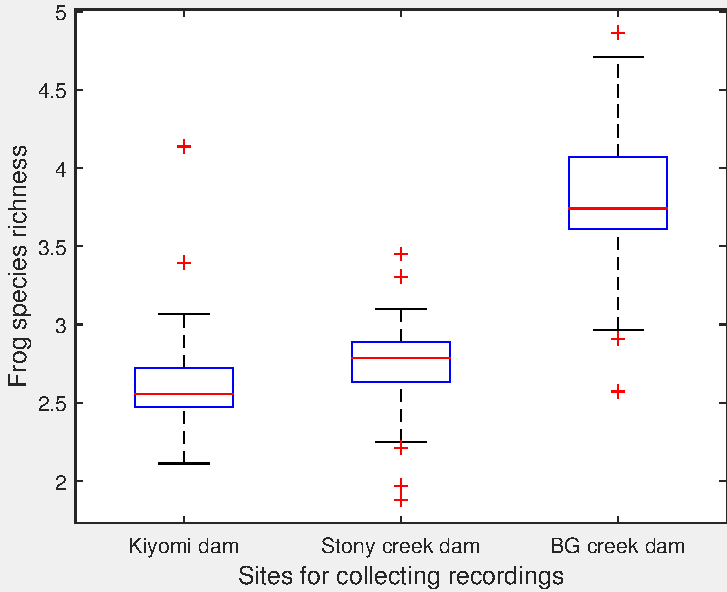
\includegraphics[width=0.5\textwidth]{image/Ch7/richnessSite.pdf}
	\caption{Averaged frog species richness of different sites.}
	\label{fig:richnessSite}
	\end{centering}
\end{figure}


\subsection{Statistical analysis}
Multiple regression analysis is used to explore frog calling activity (frog abundance and frog species richness) along weather variables (mean temperature and rainfall)\footnote[5] {http://www.bom.gov.au/?ref=hdr}. Frog calling activity is found to be highly correlated with mean temperature (F=5.18, P\textless0.05 for abundance, and F=10.7, P\textless0.01 for species richness). To calculate the correlation between rainfall and frog calling activity, we first set the rainfall vaule as the dummy variable. Then, the correlation between frog calling activity and rainfall value is also studied with multiple regression analysis (F=4.63, P\textless0.05 for abundance, and F=4.64, P\textless0.05 for species richness). The statistical analysis results indicate that frogs tend to make calls in the warm and humid environment, which is in accordance to previous studies \cite{akmentins2015patterns, canavero2008calling}.



%\begin{figure}[htb!]
%\centering
%        \begin{subfigure}[b]{0.3\textwidth}
%                \includegraphics[width=\textwidth]{image/temperature.pdf}
%                %\caption{}
%        \end{subfigure}
%       ~
%              \begin{subfigure}[b]{0.3\textwidth}
%                \includegraphics[width=\textwidth]{image/rainfall.pdf}     
%                %\caption{}           
%        \end{subfigure} 
%        \label{fig:weather}
%\end{figure}



\section{Summary and limitations}
Acoustic sensors are more widely used to monitor frog calling activity than the traditional field survey method. However, the use of acoustic sensors generates large volumes of audio data, which makes it necessary to develop automated methods. This paper proposes a novel method for detecting frog calling activity based on acoustic event detection and multi-label learning. Specifically,
acoustic event detection is the first step to calculate frog abundance. Meanwhile, each 10-second recording is analysed to decide whether it contains frog calls or not. For those recordings with frog calls, multi-label learning is further used for calculating frog species richness with multi-stage WP-based features and LPCs. Finally, statistical analysis is utilised to reflect the relationship between frog calling activity (frog abundance and frog species richness) and weather variables (mean temperature and rainfall). Experiment results show that our proposed method can accurately detect frog calling activity and reflect its relationship with weather variables. Future work will focus on a wider frog call database, including a larger number of frog species, and frog calls collected over a longer period.


